\documentclass[conference]{IEEEtran}
\IEEEoverridecommandlockouts
\usepackage{cite}
\usepackage{amsmath,amssymb}
\usepackage{graphicx}
\usepackage{stfloats}
\usepackage{pgfplots}
\pgfplotsset{compat=1.17}
\usepackage{booktabs}
\usepackage{url}
\def\BibTeX{{\rm B\kern-.05em{\sc i\kern-.025em b}\kern-.08em T\kern-.1667em\lower.7ex\hbox{E}\kern-.125emX}}

\begin{document}

\title{TremorTwin: Training a Markerless Tremor-Frequency and Severity Estimator
on a Rigged-Hand Digital Twin, with a Leakage-Controlled Evaluation}

\author{\IEEEauthorblockN{Aharshi Bhattacharjee}
\IEEEauthorblockA{\textit{North Carolina State University}\\
Raleigh, NC, USA}}

\maketitle

\begin{abstract}
Video-based tremor assessment is a promising modality for tele-neurology, but
annotated patient video is scarce and clinician ratings are subject to
inter-rater variability. This study investigates whether a model trained solely on
synthetic data can recover the two clinically relevant tremor descriptors,
oscillation frequency and severity, from hand landmarks alone. We present
TremorTwin, a landmark-level digital twin derived from an anatomically rigged hand
asset. Forward kinematics reproduce the asset's rest geometry to within
$5\times10^{-6}$ of the model size. The wrist is driven by a parametric tremor,
the moving joints are projected to image coordinates under a tracker-noise model,
and a blind estimator is trained through an iterative feature and model search. We
further identify a labelling pitfall that inflates reported accuracy: when
frequency and amplitude are both derived from a single intensity scalar, the two
prediction targets become collinear ($r=-0.97$), so an apparent joint prediction
reduces to one measurement. After the two factors are sampled independently, a
subject-held-out evaluation yields a frequency error below 1~Hz on 95.8\% of clips
(mean absolute error 0.18~Hz) and a severity grade within one grade on all clips
(exact-grade accuracy 86.5\%). A label-shuffle control returns to chance and no
subject appears in two splits. Applied to two public datasets, the same spectral
estimator recovers Parkinsonian rest-tremor frequency near 4--6~Hz and separates
patients from controls, although the separation is strong only for essential
tremor. The full landmark model has not been evaluated on real video, because the
one public dataset suited to that test is presently offline. We therefore report a
synthetic-training method, a leakage-controlled evaluation protocol, and a partial
sim-to-real result, rather than a clinical validation.
\end{abstract}

\begin{IEEEkeywords}
tremor, computer vision, hand landmarks, synthetic data, digital twin,
sim-to-real, Parkinson's disease, essential tremor
\end{IEEEkeywords}

\section{Introduction}
Tremor is among the most common movement disorders, and its two measurable
properties, oscillation frequency and amplitude, carry diagnostic and
treatment-monitoring value. In clinical practice, tremor is graded by visual
inspection using ordinal scales such as TETRAS and the MDS-UPDRS, which are
subjective and coarse. A camera-based system that tracks the hand and reports a
frequency and a severity grade would enable assessment at home between clinical
visits.

Two obstacles impede a purely data-driven approach. First, video of real patients
is difficult to obtain and to share, because faces are identifiable and the
recordings are clinical. Second, ground-truth labels are either costly
(synchronised accelerometry) or noisy (clinician grades). Synthetic data offers a
route around both constraints: a rigged hand can be oscillated at a known
frequency and amplitude and rendered as many times as required. To our knowledge,
however, no prior study trains a tremor frequency or severity model primarily on
synthetic hand data and then evaluates transfer to real patients. The most closely
related work renders a synthetic hand solely to calibrate an off-the-shelf tracker
and trains no model on it \cite{wolke2025}.

This paper pursues the synthetic-training approach and reports the conditions under
which it succeeds and fails. The contributions are as follows.
\begin{enumerate}
\item A landmark-level digital twin of a rigged hand that reproduces the source
asset's geometry exactly and injects the same parametric tremor as the underlying
rendering pipeline, so that a model can be trained without rendering any frames.
\item A measurement pitfall and its correction. Deriving tremor frequency and
amplitude from a single latent scalar renders the two targets collinear, so that a
joint prediction reduces to one measurement. We quantify the collinearity and
provide a generator that samples the two factors independently, in agreement with
the physiology \cite{pan2025}.
\item A leakage-controlled evaluation protocol, comprising subject-held-out
splits, a label-shuffle null, a train-versus-test domain check, and permutation
importance, applied to every experiment.
\item A partial sim-to-real result. The spectral core of the model recovers real
tremor frequency and separates patients from controls on two public datasets, with
the explicit caveat that this evaluates the shared signal-processing core rather
than the full landmark model.
\end{enumerate}

\section{Related Work}
\emph{Video and pose-based tremor estimation.} Pintea et al.\ estimated hand-tremor
frequency from video and released the TIM-Tremor benchmark, scoring a frequency as
correct when it falls within 1~Hz of accelerometry \cite{pintea2018}. Subsequent
work employed pose and hand-landmark trackers. G\"uney et al.\ report a frequency
error of 0.229~Hz with MediaPipe on high-frame-rate video \cite{guney2022};
Friedrich et al.\ validate a MediaPipe pipeline for frequency and amplitude against
accelerometry in 66 patients \cite{friedrich2024}; Liu et al.\ predict MDS-UPDRS
tremor scores from video \cite{liu2023}; Duque-Quiceno et al.\ score postural
tremor with a pixel-based network \cite{duque2024}. Each of these systems is
trained on real patient video.

\emph{Synthetic data and sim-to-real transfer.} Domain randomisation trains on
randomised synthetic renders so that the real world appears as one further
variation \cite{tobin2017}. Synthetic hands support generic three-dimensional
hand-pose estimation, but we found no application to a movement-disorder task.
Wolke et al.\ render an oscillating hand in Blender, but use it only to
characterise a frozen tracker rather than to train a model \cite{wolke2025}. One
digital-twin study trains exclusively on simulated tremor, but predicts muscle
activation from a wrist angle rather than frequency or severity, uses no camera,
and does not evaluate on real data. Synthetic tremor for classification has been
examined for accelerometer and EMG signals, in each case as augmentation of real
data rather than as the primary training source.

\emph{Position of this work.} The present study combines three properties that, to
our knowledge, no prior tremor study combines: a computer-vision model, trained
primarily on synthetic data, and evaluated for transfer to real patients. We
additionally report the frequency-severity collinearity, which we did not find
discussed in the tremor machine-learning literature.

\section{Method}

\subsection{Digital twin}
\begin{figure*}[t]
\centering
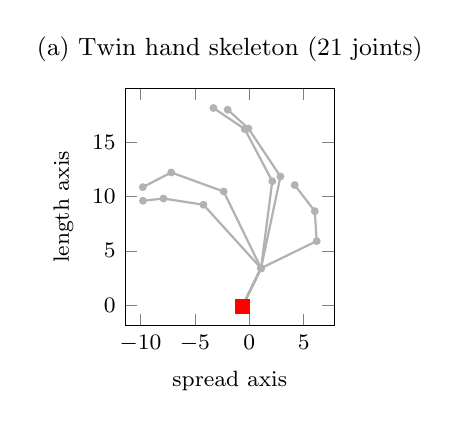
\begin{tikzpicture}
\begin{axis}[width=0.47\textwidth,height=4.6cm,axis equal image,xlabel={spread axis},ylabel={length axis},title={(a) Twin hand skeleton (21 joints)},title style={font=\small},tick label style={font=\footnotesize},label style={font=\footnotesize}]
\addplot[gray!60,thick,mark=*,mark size=1pt] coordinates {(-0.618,-0.076) (1.079,3.404) (6.197,5.898) (6.024,8.649) (4.176,11.052)};
\addplot[gray!60,thick,mark=*,mark size=1pt] coordinates {(-0.618,-0.076) (1.079,3.404) (2.865,11.837) (-0.080,16.251) (-1.989,17.980)};
\addplot[gray!60,thick,mark=*,mark size=1pt] coordinates {(-0.618,-0.076) (1.079,3.404) (2.114,11.403) (-0.421,16.201) (-3.295,18.138)};
\addplot[gray!60,thick,mark=*,mark size=1pt] coordinates {(-0.618,-0.076) (1.079,3.404) (-2.355,10.457) (-7.180,12.208) (-9.792,10.857)};
\addplot[gray!60,thick,mark=*,mark size=1pt] coordinates {(-0.618,-0.076) (1.079,3.404) (-4.216,9.240) (-7.892,9.812) (-9.777,9.609)};
\addplot[only marks,mark=square*,red,mark size=2.5pt] coordinates {(-0.618,-0.076)};
\end{axis}
\end{tikzpicture}\hfill
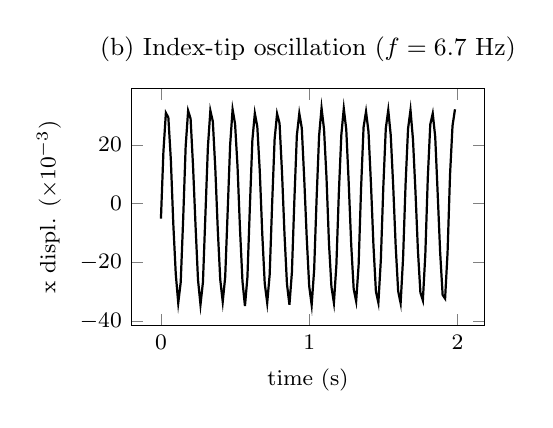
\begin{tikzpicture}
\begin{axis}[width=0.5\textwidth,height=4.6cm,xlabel={time (s)},ylabel={x displ. ($\times10^{-3}$)},title={(b) Index-tip oscillation ($f=6.7$ Hz)},title style={font=\small},tick label style={font=\footnotesize},label style={font=\footnotesize}]
\addplot[black,thick,no marks] coordinates {(0.0000,-5.0649) (0.0167,17.7394) (0.0333,30.8477) (0.0500,29.2918) (0.0667,14.9740) (0.0833,-6.8977) (0.1000,-23.9304) (0.1167,-33.7364) (0.1333,-26.7234) (0.1500,-5.1158) (0.1667,19.4390) (0.1833,31.5805) (0.2000,28.8662) (0.2167,12.5519) (0.2333,-7.4391) (0.2500,-25.8956) (0.2667,-34.3405) (0.2833,-26.6302) (0.3000,-3.6495) (0.3167,19.2435) (0.3333,31.6336) (0.3500,27.9370) (0.3667,11.8817) (0.3833,-8.7827) (0.4000,-25.8262) (0.4167,-33.3092) (0.4333,-25.0000) (0.4500,-2.7044) (0.4667,19.9545) (0.4833,32.0336) (0.5000,27.1031) (0.5167,12.4828) (0.5333,-8.7254) (0.5500,-26.4433) (0.5667,-34.7821) (0.5833,-24.9494) (0.6000,-0.7767) (0.6167,21.5411) (0.6333,30.7087) (0.6500,26.1506) (0.6667,10.9768) (0.6833,-10.1509) (0.7000,-27.0483) (0.7167,-33.6981) (0.7333,-24.1754) (0.7500,-0.0610) (0.7667,21.8678) (0.7833,30.5890) (0.8000,27.2941) (0.8167,10.4630) (0.8333,-10.2788) (0.8500,-27.2813) (0.8667,-34.3678) (0.8833,-23.3523) (0.9000,1.2488) (0.9167,23.1730) (0.9333,30.6724) (0.9500,25.6890) (0.9667,8.1916) (0.9833,-11.5066) (1.0000,-28.0418) (1.0167,-34.4053) (1.0333,-22.5050) (1.0500,1.7848) (1.0667,23.0287) (1.0833,32.5171) (1.1000,25.2971) (1.1167,8.8840) (1.1333,-13.3678) (1.1500,-28.2480) (1.1667,-33.6860) (1.1833,-20.8867) (1.2000,3.6875) (1.2167,23.3145) (1.2333,32.3496) (1.2500,25.2130) (1.2667,6.8502) (1.2833,-13.8319) (1.3000,-28.9411) (1.3167,-33.1567) (1.3333,-20.9061) (1.3500,5.3475) (1.3667,25.9671) (1.3833,31.3037) (1.4000,24.4688) (1.4167,6.6475) (1.4333,-14.0687) (1.4500,-29.7948) (1.4667,-33.6673) (1.4833,-19.0769) (1.5000,5.7778) (1.5167,25.5958) (1.5333,31.7781) (1.5500,23.2793) (1.5667,5.9118) (1.5833,-14.3374) (1.6000,-29.6444) (1.6167,-33.8286) (1.6333,-18.3912) (1.6500,6.5379) (1.6667,25.4266) (1.6833,31.8034) (1.7000,21.8254) (1.7167,4.2257) (1.7333,-15.8479) (1.7500,-30.1630) (1.7667,-32.8586) (1.7833,-17.2094) (1.8000,8.8443) (1.8167,26.9411) (1.8333,30.6420) (1.8500,22.7257) (1.8667,3.3532) (1.8833,-16.5553) (1.9000,-30.9763) (1.9167,-32.2340) (1.9333,-16.5636) (1.9500,9.8740) (1.9667,26.4417) (1.9833,32.0664)};
\end{axis}
\end{tikzpicture}
\caption{The TremorTwin digital twin. (a) The 21 rigged joints projected to two
dimensions in the hand's widest anatomical plane, forming a recognisable hand.
(b) Horizontal displacement of the index fingertip over a two-second clip, showing
the injected wrist tremor at 6.7~Hz.}
\label{fig:twin}
\end{figure*}
The source asset is a rigged hand with 21 joints, comprising a wrist and four bones
per finger. The joint hierarchy and local transforms are parsed directly from the
asset file, and joint positions are computed by forward kinematics. In the absence
of any added rotation, the computed rest positions match the asset's own scene
graph to within $5\times10^{-6}$ of the model size, which confirms the kinematics
before any dependent component is built. An anisotropic scale on the root node must
be applied for this correspondence to hold.

Only the wrist oscillates; the fingers hold a fixed configuration for the duration
of a clip. The posed hand is therefore a rigid body rotating about the wrist, which
reproduces the behaviour of the rendering pipeline that the twin represents
(Fig.~\ref{fig:twin}). At each frame the wrist rotation is set to
\begin{equation}
\theta(t) = A\left[\sin(2\pi f t) + 0.18\sin(4\pi f t + 0.5)\right] + \epsilon(t),
\end{equation}
where the second harmonic imparts a pathological waveform and $\epsilon(t)$ models
inter-cycle muscle noise. The remaining two wrist axes carry phase-shifted copies
of the same signal. All 21 joints are rotated about the wrist, projected to image
coordinates under one of four camera views, and perturbed by a MediaPipe-style
noise model comprising per-landmark jitter, whole-hand wobble, and occasional
dropped frames held at their last value.

\subsection{Two label models}
\begin{figure*}[t]
\centering
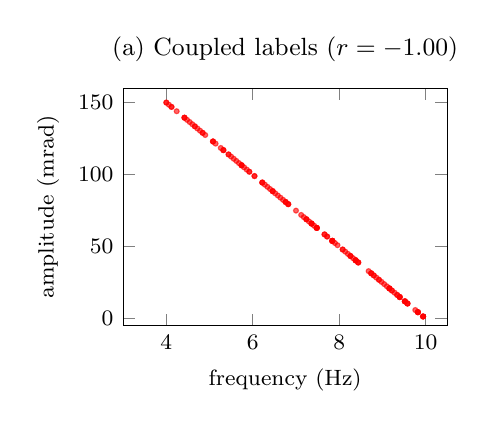
\begin{tikzpicture}
\begin{axis}[width=0.47\textwidth,height=4.6cm,xlabel={frequency (Hz)},ylabel={amplitude (mrad)},xmin=3,xmax=10.5,ymin=-5,ymax=160,title={(a) Coupled labels ($r=-1.00$)},title style={font=\small},tick label style={font=\footnotesize},label style={font=\footnotesize}]
\addplot[only marks,mark=*,mark size=0.9pt,red,opacity=0.6] coordinates {(9.520,12.000) (7.840,54.000) (5.800,105.000) (7.480,63.000) (5.740,106.500) (8.380,40.500) (5.920,102.000) (6.580,85.500) (8.680,33.000) (5.920,102.000) (9.520,12.000) (9.400,15.000) (7.480,63.000) (6.820,79.500) (7.660,58.500) (9.100,22.500) (9.820,4.500) (4.660,133.500) (5.500,112.500) (7.720,57.000) (9.580,10.500) (5.080,123.000) (9.940,1.500) (5.740,106.500) (9.820,4.500) (7.480,63.000) (6.460,88.500) (6.220,94.500) (6.220,94.500) (4.600,135.000) (9.820,4.500) (5.080,123.000) (8.200,45.000) (7.240,69.000) (7.360,66.000) (5.740,106.500) (7.360,66.000) (8.440,39.000) (9.400,15.000) (9.820,4.500) (8.920,27.000) (8.980,25.500) (9.160,21.000) (6.820,79.500) (7.840,54.000) (4.000,150.000) (7.960,51.000) (7.120,72.000) (4.480,138.000) (4.000,150.000) (9.520,12.000) (4.060,148.500) (5.560,111.000) (5.680,108.000) (4.120,147.000) (8.440,39.000) (5.320,117.000) (9.340,16.500) (6.220,94.500) (9.940,1.500) (8.260,43.500) (9.820,4.500) (8.920,27.000) (7.240,69.000) (8.260,43.500) (6.760,81.000) (8.380,40.500) (4.420,139.500) (9.400,15.000) (8.260,43.500) (5.080,123.000) (7.660,58.500) (6.820,79.500) (4.840,129.000) (6.040,99.000) (8.800,30.000) (5.620,109.500) (6.280,93.000) (8.140,46.500) (5.320,117.000) (9.940,1.500) (8.740,31.500) (9.160,21.000) (4.240,144.000) (4.120,147.000) (9.580,10.500) (4.720,132.000) (5.440,114.000) (4.840,129.000) (7.480,63.000) (4.660,133.500) (5.740,106.500) (7.180,70.500) (8.380,40.500) (5.860,103.500) (7.840,54.000) (5.260,118.500) (4.900,127.500) (9.040,24.000) (6.340,91.500) (4.780,130.500) (8.800,30.000) (7.360,66.000) (7.240,69.000) (6.520,87.000) (8.080,48.000) (6.040,99.000) (6.400,90.000) (9.280,18.000) (6.460,88.500) (9.160,21.000) (6.700,82.500) (7.360,66.000) (4.540,136.500) (5.140,121.500) (9.940,1.500) (8.740,31.500) (7.300,67.500) (8.380,40.500) (9.520,12.000) (7.000,75.000) (8.740,31.500) (6.760,81.000) (8.860,28.500) (9.220,19.500) (9.760,6.000) (8.080,48.000) (9.160,21.000) (4.420,139.500) (7.900,52.500) (7.720,57.000) (7.840,54.000) (9.220,19.500) (5.440,114.000) (8.440,39.000) (6.460,88.500) (5.320,117.000) (8.380,40.500) (7.840,54.000) (4.420,139.500) (8.320,42.000) (9.340,16.500) (9.580,10.500) (9.400,15.000) (7.840,54.000) (6.640,84.000) (7.420,64.500) (9.520,12.000) (6.760,81.000) (7.480,63.000)};
\end{axis}
\end{tikzpicture}\hfill
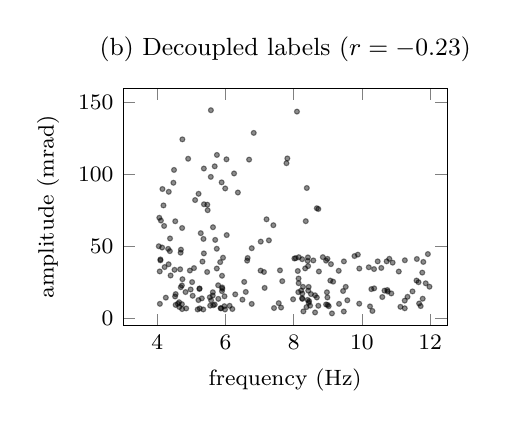
\begin{tikzpicture}
\begin{axis}[width=0.47\textwidth,height=4.6cm,xlabel={frequency (Hz)},ylabel={amplitude (mrad)},xmin=3,xmax=12.5,ymin=-5,ymax=160,title={(b) Decoupled labels ($r=-0.23$)},title style={font=\small},tick label style={font=\footnotesize},label style={font=\footnotesize}]
\addplot[only marks,mark=*,mark size=0.9pt,black,opacity=0.45] coordinates {(8.995,9.538) (4.730,62.941) (8.677,76.647) (9.922,34.781) (4.321,48.447) (5.570,98.431) (4.906,111.006) (5.790,13.753) (4.392,29.944) (10.358,21.036) (4.606,10.330) (4.338,88.071) (4.539,9.531) (6.364,87.563) (6.286,16.873) (4.830,18.471) (11.675,10.520) (5.541,14.856) (11.931,44.834) (5.241,20.994) (5.355,55.350) (5.642,9.316) (9.781,43.470) (11.978,22.175) (9.471,39.759) (4.046,50.274) (5.685,9.820) (5.634,63.471) (6.650,42.106) (11.335,15.161) (4.252,14.578) (8.948,40.250) (5.208,12.898) (6.769,10.240) (10.354,34.412) (5.579,12.672) (5.685,105.752) (9.447,19.185) (8.422,36.478) (8.271,22.096) (7.813,111.231) (4.507,33.901) (6.036,58.025) (5.897,19.089) (8.451,12.176) (4.078,10.288) (10.306,5.334) (10.756,18.775) (4.724,10.057) (5.039,15.886) (7.664,26.038) (5.699,54.682) (8.353,67.678) (4.541,17.061) (8.252,17.422) (8.409,40.113) (11.658,25.314) (4.739,27.397) (8.626,4.310) (6.122,8.917) (4.073,32.797) (6.497,13.179) (5.370,79.409) (5.972,15.525) (7.403,64.882) (4.093,41.117) (8.440,11.033) (8.722,76.138) (4.334,37.772) (8.247,41.291) (11.481,18.921) (4.957,33.401) (9.879,44.430) (9.073,26.427) (4.696,47.919) (8.987,14.737) (8.218,19.505) (5.888,94.628) (5.786,23.183) (4.730,6.649) (11.599,26.451) (4.061,70.040) (7.128,32.398) (8.374,8.032) (4.474,94.331) (5.627,16.073) (4.641,11.407) (4.375,55.669) (5.023,25.377) (7.148,21.339) (6.595,18.553) (5.630,18.346) (11.254,7.207) (8.721,8.944) (9.920,10.386) (11.127,8.210) (10.275,20.502) (7.597,33.538) (6.828,128.950) (5.326,39.619) (5.247,7.121) (5.845,39.235) (5.987,6.373) (7.273,54.368) (5.236,20.612) (5.857,7.232) (5.745,48.526) (5.992,90.395) (11.079,32.721) (9.468,4.980) (8.383,90.705) (8.948,9.850) (6.252,100.804) (8.020,41.766) (7.561,10.751) (8.505,17.084) (4.690,21.856) (5.967,8.652) (6.635,40.258) (8.119,33.088) (10.596,15.024) (5.573,144.706) (10.660,19.455) (4.492,103.251) (7.034,53.480) (4.143,49.379) (5.349,6.386) (5.212,86.675) (8.417,42.542) (4.737,124.466) (10.743,19.875) (8.973,18.321) (5.899,29.778) (8.144,24.621) (8.853,42.702) (11.869,24.558) (10.200,35.676) (7.203,68.981) (5.111,82.332) (5.908,20.761) (8.244,14.165) (9.524,22.083) (8.407,13.016) (8.738,32.769) (4.686,45.797) (10.566,35.204) (4.217,35.813) (8.989,41.529) (7.029,33.356) (10.899,38.872) (4.979,20.254) (5.478,75.303) (11.720,8.732) (4.108,68.097) (6.029,110.620) (8.134,18.424) (9.121,3.658) (4.202,64.358) (11.253,12.528) (4.723,23.066) (10.801,41.548) (8.142,27.866) (6.549,25.517) (8.095,143.730) (8.254,13.726) (5.463,32.388) (9.328,10.275) (6.202,6.694) (5.875,7.223) (5.307,14.083) (5.367,104.214) (4.523,15.395) (4.094,40.470) (11.257,40.543) (6.770,48.907) (8.438,22.017) (9.319,33.240) (4.672,34.277) (7.629,7.722) (5.276,59.361) (10.860,17.516) (8.678,14.707) (5.468,79.115) (10.461,39.773) (4.528,67.622) (5.749,113.647) (6.692,110.421) (11.780,13.836) (7.787,107.926) (10.235,8.520) (10.723,39.793) (11.608,41.410) (5.367,45.290) (4.183,78.616) (8.336,34.890) (9.571,12.752) (9.155,25.692) (4.848,7.093) (7.423,7.370) (5.746,34.799) (4.153,89.997) (5.901,21.711) (11.798,39.393) (8.575,40.411) (8.624,16.228) (8.425,19.445) (5.552,9.011) (5.185,6.378) (8.480,9.006) (4.370,46.879) (9.091,37.842) (4.647,8.122) (8.284,5.037) (8.059,42.000) (5.928,42.305) (7.982,13.460) (9.026,8.655) (11.767,31.966) (8.148,42.669) (5.078,35.099)};
\end{axis}
\end{tikzpicture}
\caption{Why the two targets must be decoupled. Each point is one synthetic clip.
(a) Under the pipeline's coupled labelling, amplitude is a deterministic function
of frequency ($r=-1.00$), so frequency and severity form a single axis. (b) Under
the decoupled generator, amplitude is sampled independently of the type-conditioned
frequency ($r=-0.23$), giving two separable targets. The gap near 6--8~Hz and the
low-amplitude cluster above 8~Hz reflect the tremor-type frequency bands.}
\label{fig:coll}
\end{figure*}
Data are generated in two configurations. The \emph{coupled} generator reproduces
the pipeline's own labelling, in which a single intensity scalar $i\in[1,100]$ sets
the frequency $f=10-0.06i$, the amplitude $A=0.0015i$, and a six-band severity
grade. Because both targets follow $i$, they are collinear (Fig.~\ref{fig:coll}a).
The \emph{decoupled} generator samples a tremor type, which fixes a frequency band
(Parkinsonian rest 4--6~Hz, essential or postural 5--9~Hz, enhanced physiologic
8--12~Hz), and samples amplitude independently; severity then follows from
amplitude, as clinical amplitude scales prescribe (Fig.~\ref{fig:coll}b). We
additionally simulate 24 to 30 subjects, each with a distinct hand shape and noise
level, so that splits may be constructed on a per-subject basis.

\subsection{Blind features}
The estimator observes only the sequence of 21 two-dimensional landmarks. For each
landmark, the two coordinate signals are high-pass filtered to remove slow drift,
after which a Welch power spectrum (dominant frequency by parabolic interpolation,
band powers, and spectral entropy) and a set of time-domain descriptors
(size-normalised displacement, jerk, zero-crossing rate, and autocorrelation
period) are computed. One feature merits explicit description: dividing a
landmark's displacement by its distance from the wrist yields the wrist rotation
amplitude directly, independently of finger configuration, camera view, and hand
size, and thus constitutes the physically appropriate severity signal. All
amplitudes are normalised by an in-clip hand size, so that camera distance does not
affect the descriptors.

\subsection{Self-improving search}
The estimator is optimised in successive rounds. Each round expands the feature set
(temporal descriptors, then spectral descriptors, then cross-landmark agreement)
and the model family (linear models, then random forests and gradient boosting,
then a tuned selection), scores each candidate by subject-grouped cross-validation,
and retains the best configuration. The procedure terminates when the score ceases
to improve. The selected model is then evaluated once on held-out subjects that
were not observed during the search.

\subsection{Leakage controls}
Every experiment applies four checks. Splits are grouped by subject, and we assert
that no subject, pose, or camera view appears in two splits. We report the
correlation between the two targets, which exposes the coupled generator. We
retrain the selected model on shuffled labels and confirm that the score returns to
chance. We train a classifier to distinguish training rows from test rows and
report its AUC. Finally, we report permutation importance to confirm that the model
relies on tremor-physics features rather than identity artifacts.

\section{Experiments and Results}

\subsection{Synthetic evaluation}
\begin{figure}[t]
\centering
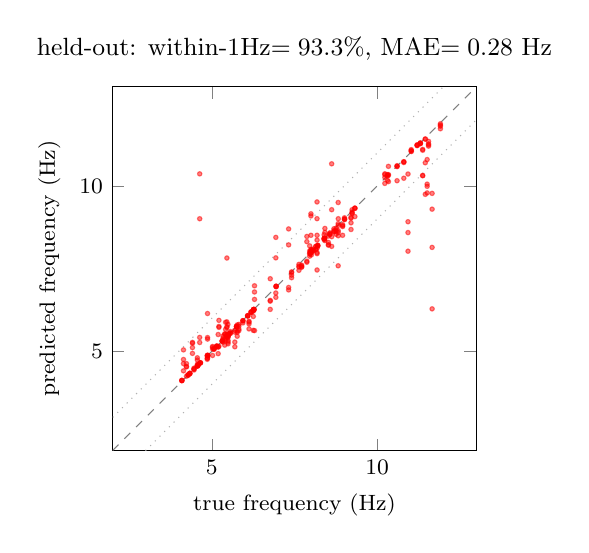
\begin{tikzpicture}
\begin{axis}[width=\columnwidth,height=6.2cm,axis equal image,xmin=2,xmax=13,ymin=2,ymax=13,xlabel={true frequency (Hz)},ylabel={predicted frequency (Hz)},title={held-out: within-1Hz$=93.3$\%, MAE$=0.28$ Hz},title style={font=\small},tick label style={font=\footnotesize},label style={font=\footnotesize}]
\addplot[gray!60,dotted] coordinates {(2,1)(13,12)};
\addplot[gray!60,dotted] coordinates {(2,3)(13,14)};
\addplot[gray,dashed] coordinates {(2,2)(13,13)};
\addplot[only marks,mark=*,mark size=0.8pt,red,opacity=0.5] coordinates {(5.558,5.597) (5.558,5.562) (5.558,5.539) (5.558,5.544) (8.420,8.716) (8.420,8.346) (8.420,8.594) (8.420,8.412) (4.653,4.651) (4.653,4.652) (4.653,4.647) (4.653,4.649) (7.975,7.965) (7.975,7.934) (7.975,7.991) (7.975,7.984) (5.022,5.122) (5.022,4.873) (5.022,5.144) (5.022,5.072) (11.211,11.241) (11.211,11.231) (11.211,11.221) (11.211,11.240) (5.416,5.877) (5.416,5.324) (5.416,5.663) (5.416,5.510) (8.759,8.538) (8.759,8.624) (8.759,8.724) (8.759,8.664) (4.335,4.322) (4.335,4.327) (4.335,4.335) (4.335,4.335) (5.314,5.308) (5.314,5.313) (5.314,5.311) (5.314,5.310) (4.461,4.489) (4.461,4.458) (4.461,4.435) (4.461,4.466) (5.696,5.136) (5.696,5.578) (5.696,5.636) (5.696,5.279) (4.563,4.558) (4.563,4.562) (4.563,4.548) (4.563,4.563) (4.586,4.588) (4.586,4.588) (4.586,4.599) (4.586,4.580) (5.491,5.225) (5.491,5.323) (5.491,5.277) (5.491,5.458) (8.145,8.076) (8.145,8.169) (8.145,8.083) (8.145,8.174) (5.066,5.081) (5.066,5.073) (5.066,5.074) (5.066,5.058) (8.822,7.586) (8.822,8.649) (8.822,9.500) (8.822,8.860) (6.260,6.254) (6.260,6.258) (6.260,6.258) (6.260,6.260) (8.568,8.534) (8.568,8.535) (8.568,8.584) (8.568,8.561) (10.807,10.234) (10.807,10.731) (10.807,10.710) (10.807,10.733) (8.956,8.508) (8.956,8.773) (8.956,8.798) (8.956,8.830) (7.996,8.019) (7.996,8.026) (7.996,8.006) (7.996,7.980) (8.527,8.292) (8.527,8.227) (8.527,8.208) (8.527,8.487) (11.914,11.842) (11.914,11.808) (11.914,11.881) (11.914,11.731) (5.940,5.858) (5.940,5.925) (5.940,5.926) (5.940,5.920) (11.555,11.205) (11.555,11.242) (11.555,11.273) (11.555,11.350) (8.182,9.011) (8.182,7.987) (8.182,9.517) (8.182,8.114) (5.503,5.507) (5.503,5.498) (5.503,5.494) (5.503,5.503) (7.874,7.725) (7.874,8.474) (7.874,8.317) (7.874,7.694) (6.125,5.827) (6.125,5.909) (6.125,5.881) (6.125,5.676) (7.716,7.551) (7.716,7.580) (7.716,7.544) (7.716,7.605) (6.187,6.188) (6.187,6.184) (6.187,6.185) (6.187,6.177) (4.282,4.280) (4.282,4.285) (4.282,4.280) (4.282,4.283) (7.635,7.574) (7.635,7.630) (7.635,7.547) (7.635,7.449) (4.633,5.419) (4.633,9.009) (4.633,10.367) (4.633,5.266) (5.748,5.747) (5.748,5.745) (5.748,5.750) (5.748,5.756) (8.397,8.382) (8.397,8.404) (8.397,8.525) (8.397,8.406) (10.934,8.591) (10.934,8.027) (10.934,8.918) (10.934,10.362) (6.255,6.053) (6.255,5.633) (6.255,6.238) (6.255,6.214) (4.862,4.757) (4.862,4.793) (4.862,4.871) (4.862,4.861) (4.870,6.142) (4.870,5.368) (4.870,5.415) (4.870,4.789) (8.825,9.010) (8.825,8.494) (8.825,8.596) (8.825,8.810) (11.457,9.747) (11.457,10.702) (11.457,11.417) (11.457,11.422) (6.085,6.076) (6.085,6.073) (6.085,6.075) (6.085,6.066) (6.944,6.968) (6.944,6.967) (6.944,6.952) (6.944,6.962) (8.063,8.041) (8.063,8.037) (8.063,8.092) (8.063,8.060) (11.307,11.289) (11.307,11.291) (11.307,11.277) (11.307,11.306) (11.032,11.099) (11.032,11.044) (11.032,11.076) (11.032,11.051) (6.291,6.981) (6.291,5.626) (6.291,6.569) (6.291,6.794) (9.242,9.173) (9.242,9.179) (9.242,9.280) (9.242,9.214) (4.414,5.244) (4.414,4.936) (4.414,5.268) (4.414,5.112) (4.562,4.803) (4.562,4.603) (4.562,4.736) (4.562,4.555) (9.014,9.038) (9.014,9.005) (9.014,8.993) (9.014,8.982) (11.378,11.107) (11.378,10.310) (11.378,10.318) (11.378,11.081) (5.149,5.160) (5.149,5.150) (5.149,5.156) (5.149,5.149) (5.390,5.528) (5.390,5.186) (5.390,5.507) (5.390,5.360) (7.412,7.403) (7.412,7.302) (7.412,7.225) (7.412,7.378) (4.875,4.863) (4.875,4.860) (4.875,4.872) (4.875,4.884) (10.233,10.369) (10.233,10.260) (10.233,10.342) (10.233,10.078) (4.143,5.042) (4.143,4.627) (4.143,4.752) (4.143,4.409) (6.275,6.264) (6.275,6.268) (6.275,6.265) (6.275,6.254) (8.694,8.609) (8.694,8.624) (8.694,8.650) (8.694,8.706) (5.819,5.814) (5.819,5.761) (5.819,5.672) (5.819,5.625) (4.094,4.117) (4.094,4.119) (4.094,4.117) (4.094,4.109) (5.768,5.572) (5.768,5.609) (5.768,5.455) (5.768,5.797) (6.936,6.632) (6.936,7.826) (6.936,8.445) (6.936,6.763) (7.323,8.218) (7.323,6.931) (7.323,8.701) (7.323,6.856) (10.311,10.169) (10.311,10.343) (10.311,10.298) (10.311,10.328) (8.012,7.988) (8.012,8.064) (8.012,8.036) (8.012,7.918) (5.455,5.490) (5.455,5.482) (5.455,5.432) (5.455,5.459) (5.487,5.526) (5.487,5.415) (5.487,5.813) (5.487,5.426) (8.406,8.393) (8.406,8.418) (8.406,8.421) (8.406,8.423) (10.603,10.159) (10.603,10.595) (10.603,10.614) (10.603,10.588) (4.232,4.527) (4.232,4.627) (4.232,4.540) (4.232,4.244) (7.960,8.188) (7.960,7.958) (7.960,7.878) (7.960,8.037) (11.513,10.056) (11.513,10.799) (11.513,9.790) (11.513,9.990) (9.210,8.885) (9.210,9.026) (9.210,8.684) (9.210,9.052) (5.339,5.461) (5.339,5.389) (5.339,5.274) (5.339,5.347) (8.183,7.459) (8.183,8.364) (8.183,8.509) (8.183,7.953) (6.767,7.195) (6.767,6.267) (6.767,6.516) (6.767,6.540) (7.998,9.159) (7.998,9.093) (7.998,8.508) (7.998,8.081) (8.204,8.196) (8.204,8.200) (8.204,8.207) (8.204,8.179) (5.215,5.751) (5.215,5.724) (5.215,5.936) (5.215,5.150) (8.625,8.173) (8.625,9.282) (8.625,10.671) (8.625,8.466) (10.342,10.132) (10.342,10.594) (10.342,10.343) (10.342,10.323) (9.327,9.325) (9.327,9.330) (9.327,9.075) (9.327,9.328) (5.456,5.717) (5.456,7.821) (5.456,5.744) (5.456,5.889) (5.192,5.507) (5.192,4.928) (5.192,5.141) (5.192,5.123) (11.663,8.142) (11.663,9.776) (11.663,9.299) (11.663,6.283)};
\end{axis}
\end{tikzpicture}
\caption{Predicted versus true tremor frequency on held-out subjects, using the
exported model (3~s clips). Most clips fall within the $\pm$1~Hz band; the residual
outliers are second-harmonic confusions and low-amplitude high-frequency clips. The
4~s configuration in Table~\ref{tab:main} reaches 95.8\% within 1~Hz.}
\label{fig:freq}
\end{figure}
Table~\ref{tab:main} reports subject-held-out results. The coupled generator
attains high nominal accuracy, placing 99.7\% of clips within 1~Hz and grading
96.9\% of clips correctly. However, the collinearity check reports $r=-0.97$
between frequency and severity (Fig.~\ref{fig:coll}a), so these two figures reflect
a single recovered quantity rather than two independent capabilities. This is the
pitfall against which the present study cautions.

Under the decoupled generator the two targets are independent ($r=0.27$), and the
resulting figures are those we regard as defensible. With 4-second clips and the
drift high-pass, the model places 95.8\% of clips within 1~Hz at a mean absolute
error of 0.18~Hz (Fig.~\ref{fig:freq}), which lies within the range reported for
real-patient MediaPipe pipelines \cite{guney2022,friedrich2024}. Severity is graded
exactly on 86.5\% of clips and within one grade on all clips; within-one-grade
accuracy is the appropriate criterion for an ordinal scale whose adjacent grades
are closely spaced \cite{zhang2021}. A signal-processing baseline, defined as the
per-axis spectral peak with no learning, already places 86.8\% of clips within
1~Hz, so learning contributes approximately nine percentage points to frequency;
the larger benefit of learning appears in severity, where amplitude must be read
through pose-dependent lever arms.

\begin{table}[t]
\caption{Subject-held-out results. ``Coupled'' denotes the pipeline's own
labelling and is included only to expose the collinearity. ``+HP'' denotes the
drift high-pass filter.}
\label{tab:main}
\centering
\setlength{\tabcolsep}{4pt}
\resizebox{\columnwidth}{!}{%
\begin{tabular}{lccccc}
\toprule
Setting & $r(f,\text{sev})$ & F$\le$1Hz & MAE & Sev & $\pm$1 \\
\midrule
Coupled, 2s      & $-0.97$ & 99.7\% & 0.14 & 96.9\% & 100\% \\
Decoupled, 2s    & 0.32 & 84.3\% & 0.49 & 81.9\% & 100\% \\
Decoupled, 4s    & 0.23 & 91.5\% & 0.27 & 90.5\% & 100\% \\
Decoupled, 4s+HP & 0.27 & 95.8\% & 0.18 & 86.5\% & 100\% \\
\bottomrule
\end{tabular}}
\end{table}

The high-pass filter introduces a trade-off between metrics. It raises frequency
accuracy from 91.5\% to 95.8\% and lowers the mean error to 0.18~Hz, but reduces
exact-grade severity by approximately four percentage points, because it attenuates
the amplitude of the slowest rest tremor near 4~Hz. Within-one-grade severity
remains at 100\%. The filter was introduced because real signals require it, as the
following subsection demonstrates.

The leakage checks pass throughout. Shuffling the labels reduces decoupled accuracy
to 0.31 against a chance rate of 0.35, and reduces the coupled case to 0.23 against
0.29, indicating that the models learn the tremor signal rather than subject
identity. No subject appears in two splits. The features on which the severity
model relies are the angular-amplitude estimate and the spectral band powers, which
is consistent with the intended design.

\subsection{Real-tremor validation}
\begin{figure*}[!b]
\centering
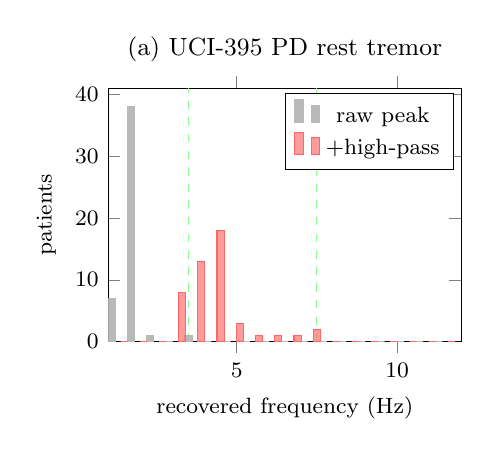
\begin{tikzpicture}
\begin{axis}[width=0.5\textwidth,height=4.8cm,ybar,bar width=2.6pt,xmin=1,xmax=12,ymin=0,ymax=41,xlabel={recovered frequency (Hz)},ylabel={patients},title={(a) UCI-395 PD rest tremor},title style={font=\small},legend style={font=\footnotesize,at={(0.98,0.98)},anchor=north east},tick label style={font=\footnotesize},label style={font=\footnotesize}]
\draw[green!45,dashed] (axis cs:3.5,0)--(axis cs:3.5,41);
\draw[green!45,dashed] (axis cs:7.5,0)--(axis cs:7.5,41);
\addplot[fill=gray!55,draw=gray!55] coordinates {(1.300,7.000) (1.900,38.000) (2.500,1.000) (3.100,0.000) (3.700,1.000) (4.300,0.000) (4.900,0.000) (5.500,0.000) (6.100,0.000) (6.700,0.000) (7.300,0.000) (7.900,0.000) (8.500,0.000) (9.100,0.000) (9.700,0.000) (10.300,0.000) (10.900,0.000) (11.500,0.000)};
\addplot[fill=red!60,draw=red!60,fill opacity=0.65] coordinates {(1.300,0.000) (1.900,0.000) (2.500,0.000) (3.100,8.000) (3.700,13.000) (4.300,18.000) (4.900,3.000) (5.500,1.000) (6.100,1.000) (6.700,1.000) (7.300,2.000) (7.900,0.000) (8.500,0.000) (9.100,0.000) (9.700,0.000) (10.300,0.000) (10.900,0.000) (11.500,0.000)};
\legend{raw peak,+high-pass}
\end{axis}
\end{tikzpicture}\hfill
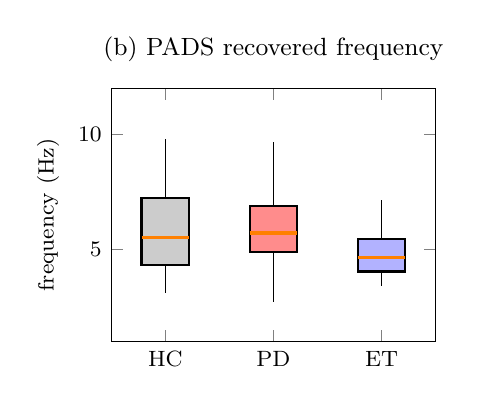
\begin{tikzpicture}
\begin{axis}[width=0.47\textwidth,height=4.8cm,xmin=0.5,xmax=3.5,ymin=1,ymax=12,xtick={1,2,3},xticklabels={HC,PD,ET},ylabel={frequency (Hz)},title={(b) PADS recovered frequency},title style={font=\small},tick label style={font=\footnotesize},label style={font=\footnotesize}]
\draw[thick,fill=gray!40] (axis cs:0.78,4.32) rectangle (axis cs:1.22,7.24);
\draw[very thick,orange] (axis cs:0.78,5.53)--(axis cs:1.22,5.53);
\draw (axis cs:1.00,7.24)--(axis cs:1.00,9.80);
\draw (axis cs:1.00,4.32)--(axis cs:1.00,3.09);
\draw[thick,fill=red!45] (axis cs:1.78,4.90) rectangle (axis cs:2.22,6.88);
\draw[very thick,orange] (axis cs:1.78,5.72)--(axis cs:2.22,5.72);
\draw (axis cs:2.00,6.88)--(axis cs:2.00,9.66);
\draw (axis cs:2.00,4.90)--(axis cs:2.00,2.74);
\draw[thick,fill=blue!30] (axis cs:2.78,4.04) rectangle (axis cs:3.22,5.45);
\draw[very thick,orange] (axis cs:2.78,4.64)--(axis cs:3.22,4.64);
\draw (axis cs:3.00,5.45)--(axis cs:3.00,7.16);
\draw (axis cs:3.00,4.04)--(axis cs:3.00,3.42);
\end{axis}
\end{tikzpicture}
\caption{Transfer of the spectral core to real tremor. (a) On UCI-395, the raw peak
sits near 2~Hz because postural drift dominates; after the same high-pass used in
training, the recovered Parkinsonian rest-tremor frequency moves into the
physiological 3.5--7.5~Hz band (shaded). (b) On PADS, recovered frequencies for
healthy controls (HC), Parkinson's disease (PD), and essential tremor (ET) are
physiological. A peak is returned even for controls, so frequency separates the
groups only weakly; detection instead relies on tremor-band power, as reported in
the text.}
\label{fig:real}
\end{figure*}
The public video dataset best suited to evaluating the full landmark model,
TIM-Tremor, is presently offline owing to a repository migration. We therefore
evaluate the shared spectral core on two public datasets in adjacent modalities,
and state explicitly that this does not evaluate the landmark model or the video
path.

\emph{UCI-395} records pen trajectories, including a task in which the patient
holds the pen on a fixed point. The hold constitutes rest tremor as a
two-dimensional position signal, which corresponds to the modality of a landmark.
Applying the model's own spectral estimator, a naive peak returns a median of
2.08~Hz, because slow postural drift dominates the raw signal. After the same
high-pass filter used in training, the recovered frequency has a median of 4.01~Hz
and falls within the 3.5--7.5~Hz band for 81\% of patients, consistent with
Parkinsonian rest tremor (Fig.~\ref{fig:real}a). The estimator separates patients
from controls with an AUC of 0.94 on peak prominence, although the control group is
small ($n=7$).

\emph{PADS} records wrist accelerometry from 469 individuals, including 79 healthy
controls, 276 with Parkinson's disease, and 28 with essential tremor. On the rest
and postural tasks the recovered frequencies lie near 5.7~Hz for both diseases,
which is physiological (Fig.~\ref{fig:real}b). The features separate essential
tremor from controls with an AUC of 0.90, which is strong; essential tremor is
defined by its postural component, so the majority of patients present a clear
signal. The features separate Parkinsonian rest tremor from controls with an AUC of
0.69. This lower value is expected rather than anomalous, and reflects a known
clinical phenomenon: a substantial proportion of Parkinson's patients are not
tremor-dominant and exhibit little rest tremor, which dilutes the group. Frequency
alone does not separate the two diseases (medians 5.7 versus 6.4~Hz, $p=0.07$),
which is likewise consistent with clinical experience.

Taken together, the two datasets indicate that the spectral core transfers to real
tremor. It recovers the correct frequency once drift is removed, and it detects
tremor strongly where tremor is the defining feature and weakly where many patients
lack it.

\section{Discussion and Limitations}
The present contribution is a method and an evaluation protocol rather than a
clinical tool, and the limitations are stated below without qualification.

The full 21-landmark model has not been evaluated on real hand video. UCI-395
provides a single landmark and PADS provides accelerometer channels, so both
evaluate the spectral core that the model shares, rather than the model itself.
Closing this gap requires real hand video with a frequency reference, which is
precisely what TIM-Tremor provided and what is currently unavailable.

The twin oscillates the wrist with the fingers held stationary. Real tremor
includes finger and pill-rolling components, so a wrist-only twin under-represents
the phenomenon. The tracker-noise model is parametric and does not reproduce real
failure modes such as self-occlusion and motion blur.

Severity estimation on real data remains largely untested. UCI-395 provides only a
patient-versus-control label with a small control group, and camera-based amplitude
is known to be less reliable than camera-based frequency \cite{wolke2025}. The
synthetic severity figures should therefore be interpreted as an upper bound under
ideal tracking.

Two of the works against which we position this study were behind paywalls, so
those statements rest on abstracts and should be verified before a camera-ready
version.

\section{Conclusion}
We trained a hand-tremor frequency and severity estimator on a rigged digital twin
and evaluated it under a leakage-controlled protocol. On decoupled,
subject-held-out synthetic data the model attains a frequency error of 0.18~Hz and
grades severity within one grade on all clips, with the leakage controls passing
throughout. The same spectral core recovers real Parkinsonian rest-tremor frequency
near 4~Hz and separates essential-tremor patients from controls at an AUC of 0.90
on two public datasets. In the course of this work we identified and corrected a
labelling pitfall that would otherwise have reduced a joint frequency-and-severity
claim to a single measurement. The remaining step is a real-video evaluation of the
full landmark model, for which the software is in place and only suitable data is
lacking.

\begin{thebibliography}{00}
\bibitem{pintea2018} S.~L. Pintea, J. Zheng, X. Li, P.~J.~M. Bank, J.~J. van
Hilten, and J.~C. van Gemert, ``Hand-tremor frequency estimation in videos,'' in
\emph{Proc. ECCV Workshops}, 2018, arXiv:1809.03218.
\bibitem{guney2022} G.~G\"uney \emph{et al.}, ``Video-based hand movement analysis
of Parkinson patients using high-frame-rate videos and MediaPipe,'' \emph{Sensors},
vol.~22, no.~20, p.~7992, 2022.
\bibitem{friedrich2024} M.~U. Friedrich \emph{et al.}, ``Validation and application
of computer vision algorithms for video-based tremor analysis,'' \emph{npj Digital
Medicine}, vol.~7, p.~165, 2024.
\bibitem{liu2023} W.~Liu \emph{et al.}, ``Vision-based estimation of MDS-UPDRS
scores for quantifying Parkinson's disease tremor severity,'' \emph{Medical Image
Analysis}, vol.~85, p.~102754, 2023.
\bibitem{duque2024} F.~Duque-Quiceno, G. Sarapata, Y. Dushin, M. Allen, and J.
O'Keeffe, ``Deep learning for objective estimation of Parkinsonian tremor
severity,'' arXiv:2409.02011, 2024.
\bibitem{zhang2021} L.~Zhang, V. Yadav, V. Koesmahargyo, A. Abbas, and I.
Galatzer-Levy, ``Prediction of clinical tremor severity using rank consistent
ordinal regression,'' arXiv:2105.01133, 2021.
\bibitem{wolke2025} R.~Wolke, J. Welzel, W. Maetzler, G. Deuschl, and J. Becktepe,
``Validity of tremor analysis using smartphone compatible computer vision
frameworks,'' \emph{Scientific Reports}, vol.~15, no.~1, p.~13391, 2025.
\bibitem{tobin2017} J.~Tobin, R. Fong, A. Ray, J. Schneider, W. Zaremba, and P.
Abbeel, ``Domain randomization for transferring deep neural networks from
simulation to the real world,'' in \emph{Proc. IEEE/RSJ IROS}, 2017, pp.~23--30.
\bibitem{pan2025} M.-K. Pan, ``Targeting the fundamentals for tremors: the
frequency and amplitude coding in essential tremor,'' \emph{Journal of Biomedical
Science}, vol.~32, p.~18, 2025.
\bibitem{pads2023} J.~Varghese \emph{et al.}, ``Predicting Parkinson's disease
using smartwatch sensor data (PADS),'' PhysioNet, 2023.
\bibitem{uci395} M.~E. Isenkul, B.~E. Sakar, and O. Kursun, ``Improved spiral test
using digitized graphics tablet for monitoring Parkinson's disease,'' UCI Machine
Learning Repository, dataset~395.
\end{thebibliography}

\end{document}
